\documentclass[epsf]{article}
\usepackage{amsmath,amsthm,amsfonts,latexsym,amscd, framed}
\usepackage{graphicx}
%\title{Project \#2: The Accumulation Function}
%\date{Solutions due Friday, October 12th}

\textwidth=6.0truein\hoffset=-.5truein
\textheight=8.5truein\voffset=-.5truein

\begin{document}
%\maketitle
\newcommand{\R}{\mathbb{R}}
\newcommand{\noi}{\noindent}
\newcommand{\bs}{\bigskip}

%%%%


\begin{center}
{\Large Project \#1: Undoing the Chain Rule\\
\vskip 2mm
Pre-Work}
\end{center}


\noi{\bf PW 1}  Recall that the circle of radius $2$ centered at $(1,3)$
is described in the plane by the equation
$(x-1)^2+(y-3)^2=4.$
\begin{itemize}
\item[(a)]  This equation does {\bf not} define a function.  Why?

\item[(b)]  However, the equation for a circle can be used to define several functions {\em implicitly}.  What do you think this means?

\item[(c)] Use the chain rule to find the slope of a tangent line at a fixed point $(x_0, y_0)$ of the graph of
one of these implicit functions.  \\
\end{itemize}

\noi{\bf PW 2} The graph of the equation $y^2=x^3-x$ is a famous elliptic curve related to the proof of Fermat's Last Theorem\footnote{see http://en.wikipedia.org/wiki/Fermat}. 

\begin{itemize}
\item[(a)] Give a formula for the slope of a tangent line to any point $(x_0, y_0)$ of this curve.  Where are the tangents vertical?

\item[(b)] Suppose a function $f(x)$ is implicitly defined by the curve $y^2=x^3-x$.  What differential equation
does $f(x)$ satisfy? 

\item[(c)] Sketch the slope-field for the differential equation in (b). Plot the elliptic curve
$y^2=x^3-x$ on the same plane.  You can use the grid on the back of this page for your slope field.

\item[(d)] Does the differential equation you came up with in part (b) have any solutions that aren't defined implicitly by the curve $y^2=x^3-x$?  If so, sketch one of these solutions on your slope-field.  If not, explain.
\end{itemize}

\newpage


Use the dot grid below to sketch your slope field for PW 2 (c).  Sketch a dash at each $(x,y)$ gridpoint whose slope matches the value of $y'$ for the corresponding values of $(x,y)$. \\

You may find it helpful to make a table of $x$, $y$ and $y'$ values and take advantage of any symmetry you notice.
\vskip 1 in
\begin{center}
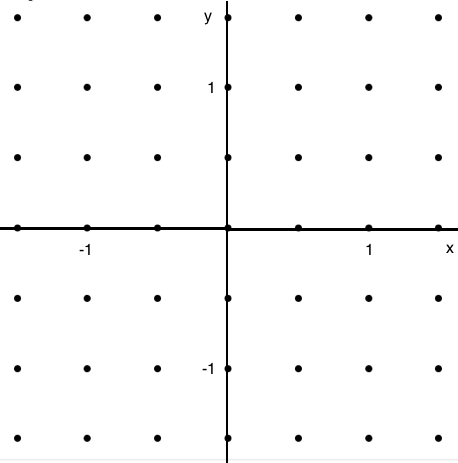
\includegraphics[width=100mm]{dotgrid.png}
\end{center}

\end{document}